
%==========================================================================================================
% MULAI BAB III
%==========================================================================================================
\chapter{PERANCANGAN DAN IMPLEMENTASI}
\label{chap:implementasi}
%==========================================================================================================
% Subbab
%==========================================================================================================
\section{Teknologi}
\label{sec:teknologi_implementasi}

\subsection {\textit{Rich Internet Application} (RIA)}
\label{subsec:RIA}
Rich Internet applications (RIAs) are web applications that have most of the characteristics of desktop applications, typically delivered either by way of a standards based web browser, via a browser plug-in, or independently via sandboxes or virtual machines.[1] Examples of RIA frameworks include Ajax, Curl, GWT, Adobe Flash/Adobe Flex/AIR, Java/JavaFX,[2], Mozilla's XUL and Microsoft Silverlight.[3]

The term was introduced in March 2002 by vendors like Macromedia who were addressing limitations at the time in the "richness of the application interfaces, media and content, and the overall sophistication of the solutions" by introducing proprietary extensions.[4] There has been some debate about whether Ajax properly qualifies as an RIA or whether the term should be reserved for plug-in based technologies. However Ajax clearly demonstrates all the core characteristics of an RIA and current opinion appears to hold that it should be therefore be included in this category[5].

As web standards have developed and the compliance of web browser has improved, the need for plug-in based RIAs has diminished. The rapid evolution of Javascript and the emergence of a broad range of Ajax-based desktop-like widget sets have continued this trend. HTML 5 takes this even further by delivering an extensive pseudo-application platform. [6]

With a few but growing number of exceptions (most notably YouTube which currently relies on Adobe Flash for video playback) the vast majority of the most popular web sites are native web applications. However, many major sites make use of RIA frameworks such as Ajax and Adobe Flash. Online gaming is an area where plugin-based RIAs are particularly prevalent. Applications (such as Dimdim) which require access to video capture also tend to use RIAs (with the notable exception of Gmail which uses its own task-specific browser plug-in[7]).

\subsubsection {Adobe Flash}
\label{subsubsec:adobe_flash}
Adobe Flash (formerly Macromedia Flash) is a multimedia platform originally acquired by Macromedia and currently developed and distributed by Adobe Systems. Since its introduction in 1996, Flash has become a popular method for adding animation and interactivity to web pages. Flash is commonly used to create animation, advertisements, and various web page Flash components, to integrate video into web pages, and more recently, to develop rich Internet applications.

Flash can manipulate vector and raster graphics, and supports bidirectional streaming of audio and video. It contains a scripting language called ActionScript. Several software products, systems, and devices are able to create or display Flash content, including Adobe Flash Player, which is available free for most common web browsers, some mobile phones and for other electronic devices (using Flash Lite). The Adobe Flash Professional multimedia authoring
program is used to create content for the Adobe Engagement Platform, such as web applications, games and movies, and content for mobile phones and other embedded devices.

Files in the SWF format, traditionally called "ShockWave Flash" movies, "Flash movies" or "Flash games", usually have a .swf file extension and may be an object of a web page, strictly "played" in a standalone Flash Player, or incorporated into a Projector, a self-executing Flash movie (with the .exe extension in Microsoft Windows or .hqx for Macintosh). Flash Video files have a .flv file extension and are either used from within .swf files or played through a flv-aware player, such as VLC, or QuickTime and Windows Media Player with external codecs added.

\subsubsection {Adobe Flex}
\label{subsubsec:adobe_flash}
Adobe Flex is a software development kit released by Adobe Systems for the development and deployment of cross-platform rich Internet applications based on the AdobeFlash platform. Flex applications can be written using Adobe Flex Builder or by using the freely available Flex compiler from Adobe.

Traditional application programmers found it challenging to adapt to the animation metaphor upon which the Flash Platform was originally designed. Flex seeks to minimize this problem by providing a workflow and programming model that is familiar to these developers. MXML, an XML-based markup language, offers a way to build and lay out graphic user
interfaces. Interactivity is achieved through the use of ActionScript, the core language of Flash Player that is based on the ECMAScript standard.

The Flex SDK comes with a set of user interface components including buttons, list boxes, trees, data grids, several text controls, and various layout containers. Charts and graphs are available as an add�]on. Other features like web services, drag and drop, modal dialogs, animation effects, application states, form validation, and other interactions round out the application framework.

In a multitiered model, Flex applications serve as the presentation tier. Unlike pagebased HTML applications, Flex applications provide a stateful client where significant changes to the view don't require loading a new page. Similarly, Flex and Flash Player provide many useful ways to send and load data to and from server-side components without requiring the client to reload the view. Though this functionality offered advantages over HTML and JavaScript development in the past, the increased support for XMLHttpRequest in major browsers has made asynchronous data loading a common practice in HTML-based development as well.

\subsubsection {Action Script}
\label{subsubsec:action_script}
ActionScript is a scripting language based on ECMAScript. ActionScript is used primarily for the development of websites and software using the Adobe Flash Player platform (in the form of SWF files embedded into Web pages), but is also used in some database applications (such as Alpha Five), and in basic robotics, as with the Make Controller Kit. Originally developed by Macromedia, the language is now owned by Adobe (which acquired Macromedia in 2005). ActionScript was initially designed for controlling simple 2D vector animations made in Adobe Flash (formerly Macromedia Flash). Later versions added functionality allowing for the creation of Web-based games and rich Internet applications with streaming media (such as video and
audio).

\subsubsection {Adobe Flash Builder}
\label{subsubsec:adobe_flash_builder}
Flash Builder 4 is Adobe's professional Flex IDE built on Eclipse. It can run either as astandalone tool or as a plugin to an existing Eclipse installation. Flex SDK includes the Flex framework (also known as the Flex class library), Flex command-line compilers, Adobe Integrated Runtime (AIR) framework, Adobe AIR command-line compilers, the Flex debugger,
the ASDoc utility, and the debugger version of Flash Player. Use the Flex SDK to develop, compile, and deploy Flex applications that connect to XML and SOAP web services with no additional charges or server licensing required. This release also includes Data Visualization features.

\subsection {ARToolKit}
\label{subsec:artoolkit}
ARToolKit is a C and C++ language software library that lets programmers easily develop Augmented Reality applications. ARToolKit was originally developed by Dr. Hirokazu Kato, and its ongoing development is being supported by the Human Interface Technology Laboratory (HIT Lab) at the University of Washington, HIT Lab NZ  at the University of Canterbury, New Zealand, and ARToolworks, Inc, Seattle.

One of the most difficult parts of developing an Augmented Reality application is precisely calculating the user's viewpoint in real time so that the virtual images are exactly aligned with real world objects. ARToolKit uses computer vision techniques to calculate the real camera position and orientation relative to marked cards, allowing the programmer to overlay virtual objects onto these cards. The fast, precise tracking provided by ARToolKit should enable the rapid development of many new and interesting AR applications. \sout{ARToolKit uses computer vision algorithms to solve this problem. The ARToolKit video tracking libraries calculate the real camera position and orientation relative to physical markers in real time. This enables the easy development of a wide range of Augmented Reality applications.} Some of the features of ARToolKit include:

\begin{itemize}
	\item Single camera position/orientation tracking.
  \item Tracking code that uses simple black squares.
  \item The ability to use any square marker patterns. 
  \item Easy camera calibration code.
  \item Fast enough for real time AR applications.
  \item SGI IRIX, Linux, MacOS and Windows OS distributions.
  \item Distributed with complete source code.
\end{itemize}

ARToolKit currently runs on the SGI IRIX, PC Linux, Mac OS X, and PC Windows (95/98/NT/2000/XP) operating systems. The last version of ARToolKit is completly multi-platform. The functionality of each version of the toolkit is the same, but the performance may vary depending on the different hardware configurations. 

\subsubsection{Prinsip Kerja ARToolKit}
\label{subsubsec:prinsip_artoolkit}
ARToolKit applications allow virtual imagery to be superimposed over live video of the real world. Although this appears magical it is not. The secret is in the black squares used as tracking markers. The ARToolKit tracking works as follows:
   
\begin{enumerate}
	\item The camera captures video of the real world and sends it to the computer.
	\item Software on the computer searches through each video frame for any square shapes
	\item If a square is found, the software uses some mathematics to calculate the position of the camera relative to the black square.
	\item Once the position of the camera is known a computer graphics model is drawn from that same position.
	\item This model is drawn on top of the video of the real world and so appears stuck on the square marker.
	\item The final output is shown back in the handheld display, so when the user looks through the display they see graphics overlaid on the real world.
\end{enumerate}

\begin{figure}
	\centering
		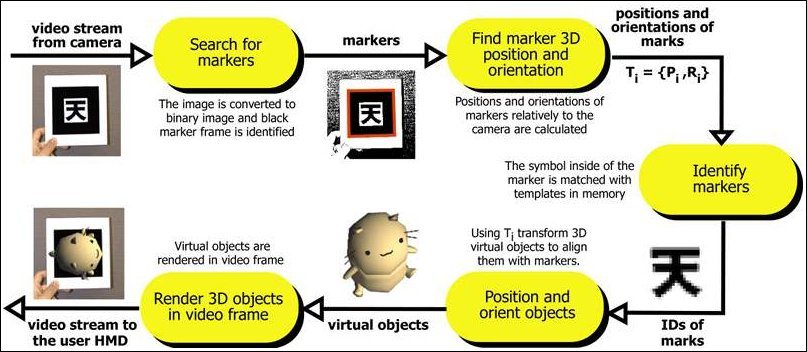
\includegraphics[width=14cm]{images/diagram_artoolkit.jpg}
	\caption{Diagram ARToolKit}
	\label{fig:diagram_artoolkit}
\end{figure}

The figure \ref{fig:diagram_artoolkit} summarizes these steps. ARToolKit is able to perform this camera tracking in real time, ensuring that the virtual objects always appear overlaid on the tracking markers. 

\subsection {FLARToolKit}
\label{subsec:FLARToolKit}
Back in November 2008, a group of Japanese coders, working largely under the radar, unveiled a project that redefined many ActionScript developers' ideas of what the language could do. FLARToolKit, developed primarily by Tomohiko Koyama (aka Saqoosha), introduced  augmented reality to the web, and to a large segment of the population as a whole.

FLARToolKit is the latest in a series of ports of ARToolkit \sout{,an augmented reality C++ library originally developed by Dr. Hirokazu Kato at the Human Interface Technology Lab at University of Washington}. With the advent of ActionScript 3.0, developers like Mario Klingemann and others began experimenting with realtime image analysis techniques for Flash Player. Saqoosha picked up on this, and ported FLARToolKit from NYARToolkit, a Java/C-\sout{sharp}/Android port of ARToolkit. 

FLARToolKit made its biggest initial splash at the hands of North Kingdom, the Swedish interactive agency that developed GE's SmartGrid augmented reality campaign. Since then, a host of AR applications have made their way to the web via FLARToolKit; the majority of them are variations on the theme of 3D characters dancing on top of live video, or games. As time goes on, however, creative developers will imagine new, creative, and useful applications of the technology.

\subsection {The FLARToolKit process}
\label{subsec:FLARToolKit}
FLARToolKit does the following steps to create final AR image.
\begin{enumerate}
	\item Capture the image from webcam.
	\item Binarize input image (thresholding).
	\item Labeling.
	\item Find squares.
	\item Matching with patterns.
	\item Calculate transform matrix.
	\item Render the 3D objects.
\end{enumerate}

\subsubsection {\textit{Thresholding}}
\label{subsubsec:thresholding}
The first step in many computer vision applications that rely on edge detection is to  threshold the source image. A binary image is made by changing pixels brighter than a threshold value to one color, and pixels darker than the threshold to another. 
\begin{figure}[h]
\begin{center}
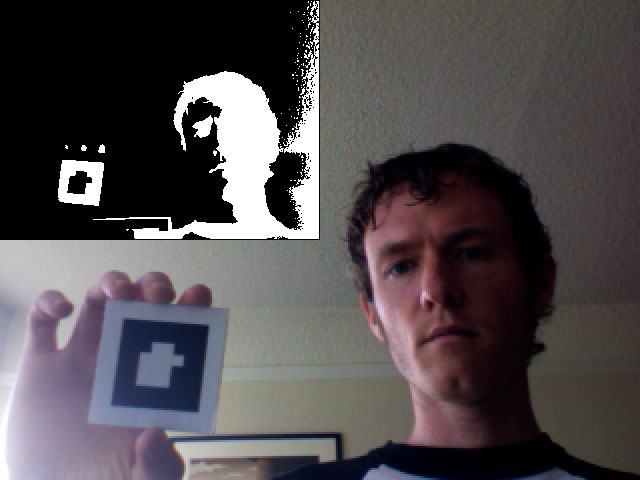
\includegraphics[width=7cm]{./images/thresholding}
\caption{\label{fig:thresholding} Thresholding}
\end{center}
\end{figure}
Thresholding separates the source image into a binary image, making analysis less computationally expensive.

\subsubsection {\textit{Labeling}}
\label{subsubsec:labeling}
FLARToolKit's next step is to find contiguous areas in the thresholded image, speficially within the areas below the threshold (darker areas). Using BitmapData.getColorBoundsRect and BitmapData.floodFill, contiguous areas are 'labeled' with unique colors, used later to id the areas.
\begin{figure}[h]
\begin{center}
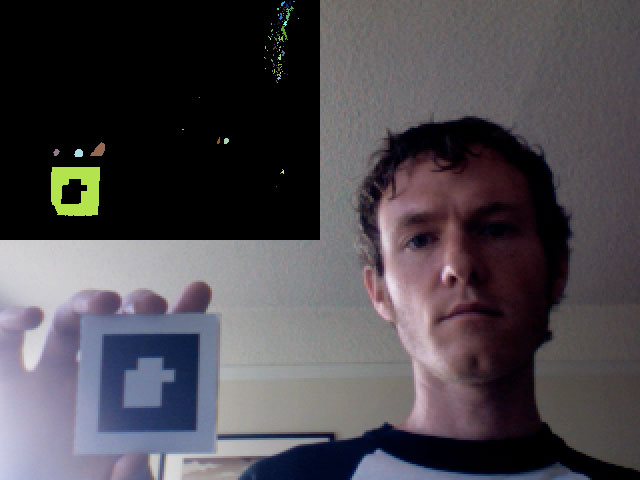
\includegraphics[width=7cm]{./images/labeling}
\caption{\label{fig:labeling} Each contiguous area of white (corresponding to dark areas of the source image) is 'labeled' with a different color. }
\end{center}
\end{figure}

\subsubsection {Marker Outline Detection}
\label{subsubsec:labeling}
With candidates for marker locations, FLARToolKit then proceeds to search the labeled areas for shapes that could be transformed squares (i.e. marker outlines). 

\subsubsection {Pattern Matching}
\label{subsubsec:pattern_matching}
Once all marker outline possibilities have been established, FLARToolKit analyzes the areas of the image within the outlines and compares the contents with the list of patterns the developer has asked FLARTookit to detect. FLARToolKit assigns a 'confidence' value to all of the matches; matches that are at or above the confidence level specified by the developer are reported as pattern matches. 

\subsection {Papervision 3D}
\label{subsec:papervision3D}
Papervision3D is an open source 3D engine for the Flash platform.

\section {Augmented Reality (AR) menggunakan FLARToolKit dan Papervision3D}
\label{sec:AR_flar_PV3D}
AR is combining real world objects with virtual  ones (computer generated). Major experimentation with AR has been in field of video processing, where live video feeds are combined with 2D or 3D objects. In Flash, this is usually done with a webcam and a marker card. When you hold the card up to the webcam, Flash is able to detect the orientation of the marker and superimpose, in this case, a 3d model on top of it. This technology has been around for a while now and having access to it in Flash is really exciting. Although it is still in its infancy, over time the speed and power of AR will improve to hopefully play an important role in how we view the web.

\section {Perancangan Aplikasi}
\label{sec:perancangan}